% Copyright 2024 Fausto Spoto
%
% Licensed under the Apache License, Version 2.0 (the "License");
% you may not use this file except in compliance with the License.
% You may obtain a copy of the License at
%
%    http://www.apache.org/licenses/LICENSE-2.0
%
% Unless required by applicable law or agreed to in writing, software
% distributed under the License is distributed on an "AS IS" BASIS,
% WITHOUT WARRANTIES OR CONDITIONS OF ANY KIND, either express or implied.
% See the License for the specific language governing permissions and
% limitations under the License.

\documentclass[11pt]{beamer}  %% versione proiettore
%%\documentclass[11pt,handout]{beamer} %% versione stampa
\usepackage{lucidiJb-2ed}

\usepackage{mathtools}
\usepackage{relsize}
\usepackage[normalem]{ulem}

\mode<article>
{
  \usepackage{fullpage}
  \usepackage{hyperref}
}

\mode<presentation>
{
  \setbeamertemplate{background canvas}[vertical shading][bottom=red!10,top=blue!10]
  \usetheme{Course}
  \usefonttheme[onlysmall]{structurebold}
}

\subtitle{S\~ao Luis, Brasil, 18/6/2024}
\title{Blockchain and its Energy Cost}
\institute{Universit\`a di Verona, Italy}
\date{June 2024}

\setbeamercovered{invisible}

\def\codesize{\smaller}
\def\<#1>{\codeid{#1}}
\newcommand{\codeid}[1]{\ifmmode{\mbox{\codesize\ttfamily{#1}}}\else{\codesize\ttfamily #1}\fi}

\AtBeginSection[]{
  \begin{frame}
  \vfill
  \centering
  \begin{beamercolorbox}[sep=8pt,center,shadow=true,rounded=true]{title}
    \usebeamerfont{title}\insertsectionhead\par%
  \end{beamercolorbox}
  \vfill
  \end{frame}
}

\begin{document}

\begin{frame}
  \titlepage
\end{frame}

\begin{frame}\frametitle{Who issues and moves the money?}

  \begin{center}
    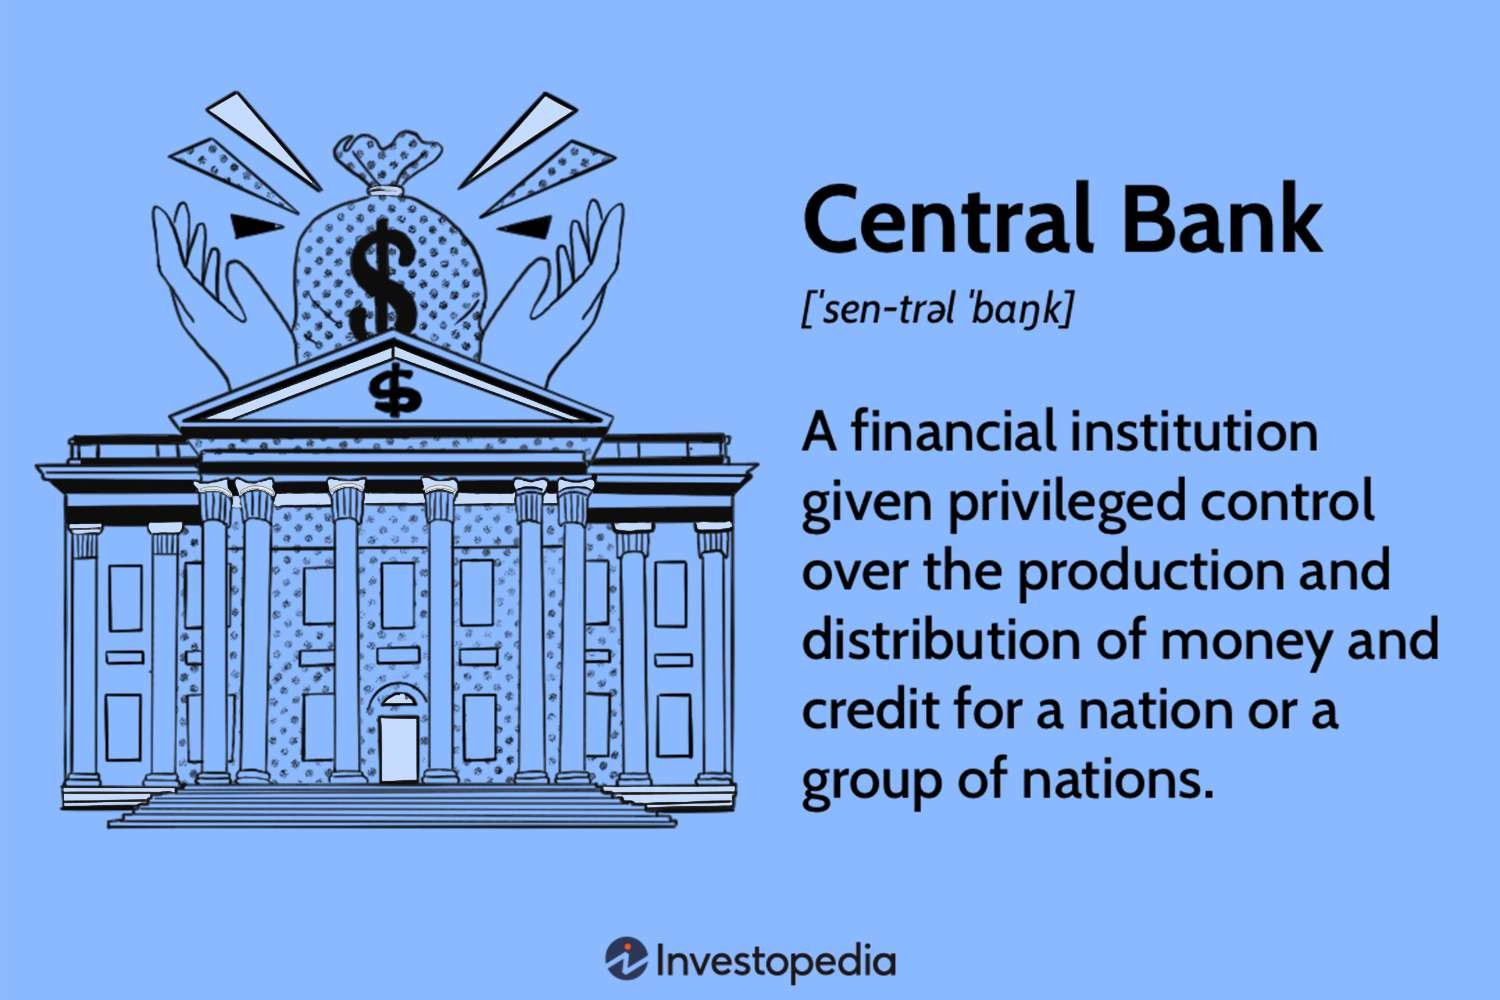
\includegraphics[scale=0.22,clip=false]{pictures/central-bank.jpg}
  \end{center}

\end{frame}

\begin{frame}\frametitle{Can I at least move the money?}

  \begin{center}
    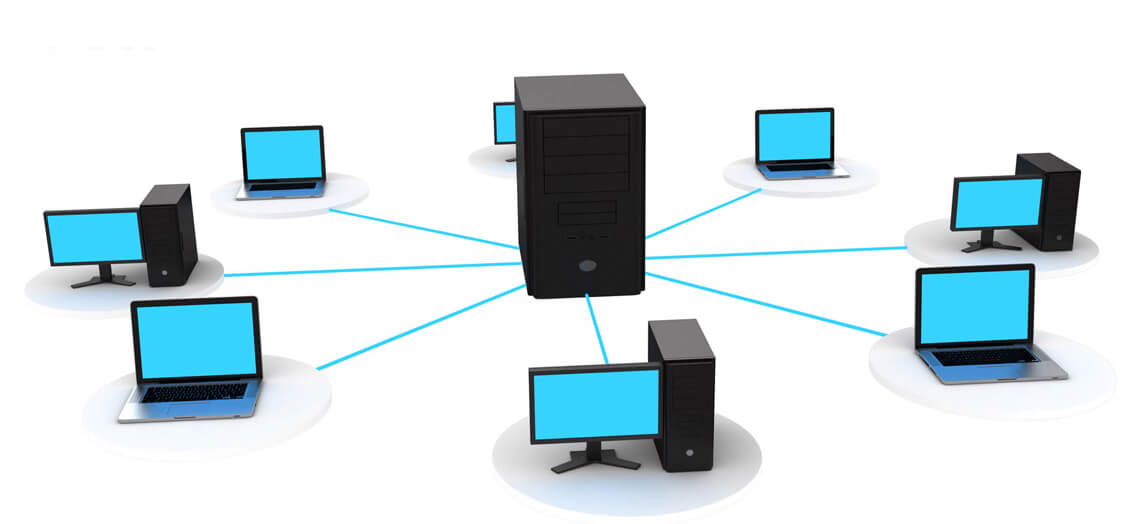
\includegraphics[scale=0.22,clip=false]{pictures/centralized-network.jpg}
  \end{center}

  \begin{greenbox}{It's all about trust}
    \begin{itemize}
    \item if my central computer crashes, data might get lost
    \item if I modify the data in my central computer, I modify
      the accounts of the users
    \end{itemize}
  \end{greenbox}
  
\end{frame}

\begin{frame}{Trust is rare in this world}

  \begin{itemize}
  \item we trust our supermarket points because they have little and limited value
  \item we trust PayPal because we keep and exchange little money on it
  \item we trust credit card issuers up to a few thousand dollars
    because they \emph{should not} fail
    and \emph{should not} cheat (too big to fail, to big to cheat)
  \end{itemize}

\end{frame}

\begin{frame}\frametitle{Can trust arise in a trusteless world?}

  \begin{greenbox}{We want a money handling system that}
    \begin{itemize}
    \item has no central, special computer
    \item consists of many computers, all created equal
    \item if some computers fail, the network survives
    \item each computer contains all data, it does not need the others
    \item if a computer holds corrupted data, we can immediately see it
    \item each single computer is very unlikely to change its data
      from a non-corrupted state to another non-corrupted state (history
      must be hard to change, no double spending)
    \end{itemize}
  \end{greenbox}

  \begin{center}
    
\includegraphics[scale=0.3,clip=false]{pictures/unicorn.jpg}
  \end{center}

\end{frame}

\begin{frame}\frametitle{Distributed network}

  \begin{center}
    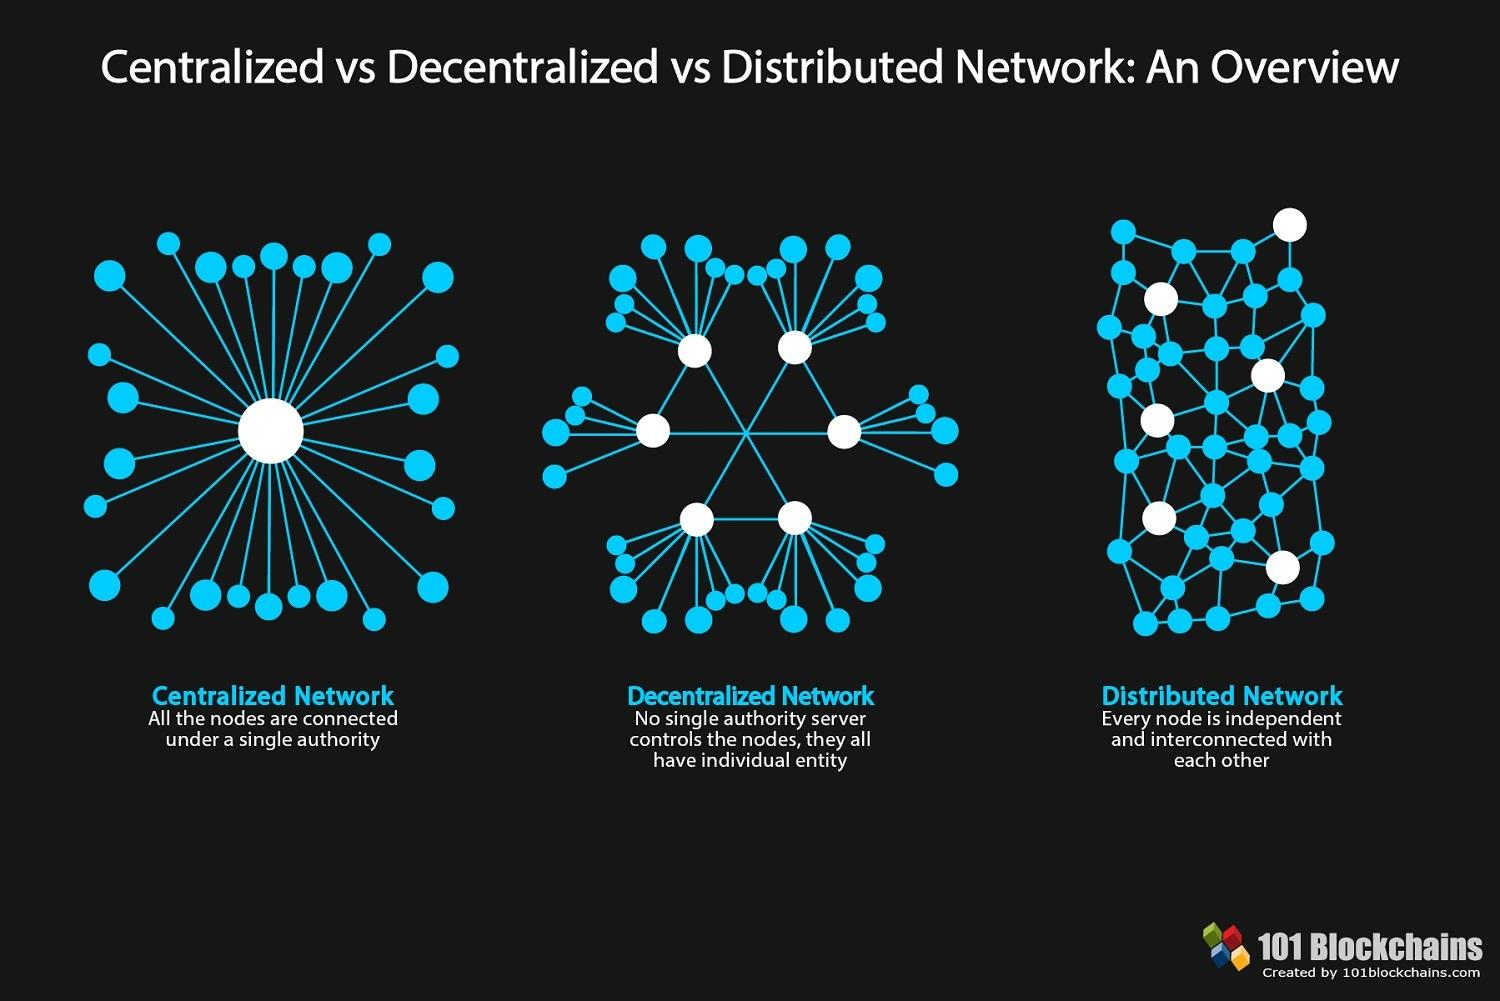
\includegraphics[scale=0.22,clip=false]{pictures/distributed.jpg}
  \end{center}

\end{frame}

\begin{frame}\frametitle{A Bit of History}

  \begin{itemize}
  \item[1991] a cryptographically secure chain of blocks (Haber \& Stornetta)
  \item[1992] proof of work (Dwork \& Naor)
  \item[2008] the sum of the above two becomes Bitcoin (Nakamoto)
  \end{itemize}

  \bigskip

  \begin{greenbox}{Why did it take so long?}
    \begin{itemize}
    \item because researchers live in isolated bubbles
    \item because the implementation was complicated
    \end{itemize}
  \end{greenbox}

\end{frame}

\begin{frame}\frametitle{A Secure Chain of Blocks}

  \begin{center}
    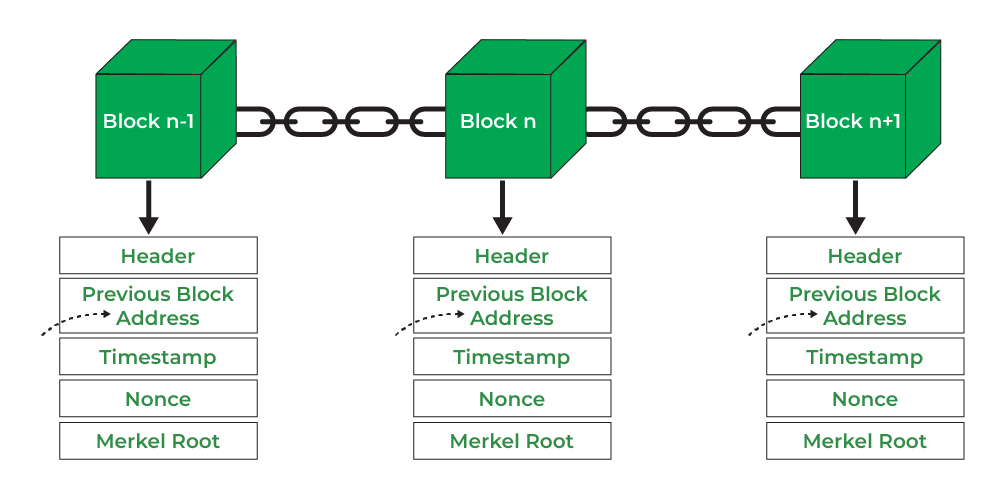
\includegraphics[scale=0.26,clip=false]{pictures/blocks.png}
  \end{center}

  If one modifies data in block $n$, then also blocks $n+1$, $n+2$, \ldots
  must be modified because otherwise the previous hash links do not match

  \medskip

  \begin{redbox}{}
    It's still possible in a few seconds for a modern computer
  \end{redbox}
  
\end{frame}

\begin{frame}\frametitle{Proof of Work}

  \begin{redbox}{}
    Cynthia Dwork and Noni Naor (1992). “Pricing via Processing, Or, Combatting Junk Mail, Advances in Cryptology”. CRYPTO’92: Lecture Notes in Computer Science No. 740. Springer: 139–147.
  \end{redbox}

  \bigskip

  \begin{tabular}{ccc}
    text of email & hashing & \\
    recipient address & $\Rightarrow$ & $\mathtt{\underbrace{0000000}43f5e6bc00d56984\ldots5974edf}$\\
    date of the email && \\
    numerical nonce &&
  \end{tabular}

  \bigskip

  The email client will accept the email only if the hash starts with at least 7 (or more) zeros

  \bigskip

  The sender needs to try and retry the hashing by changing the nonce, until it finds a good hash that will be accepted

  \bigskip

  This takes time and consumes energy: it makes spam expensive

\end{frame}

\begin{frame}\frametitle{Bitcoin = Secure chain of blocks + Proof of work}

  \begin{center}
    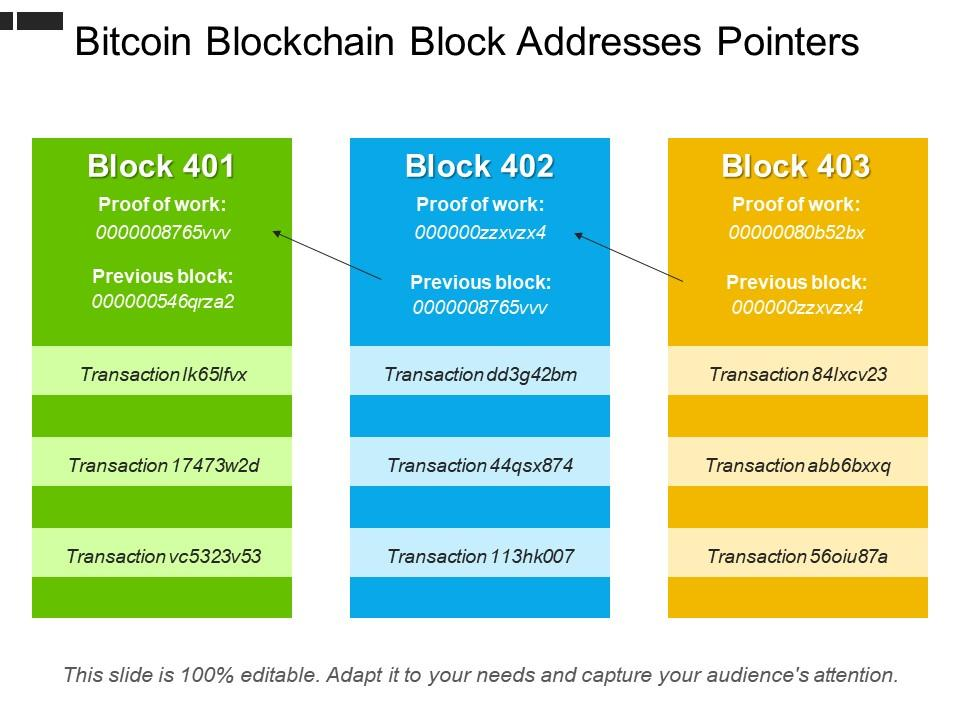
\includegraphics[scale=0.28,clip=false]{pictures/blocks-pow.jpg}
  \end{center}

  \begin{redbox}{}
    If one modifies data in block $n$, then also blocks $n+1$, $n+2$, \ldots
    must be modified because otherwise the previous hash links do not match
    and their proof of block must be recomputed: it takes centuries even on
    a very fast computer
  \end{redbox}

\end{frame}

\begin{frame}\frametitle{How to kill a dictator}

  \begin{greenbox}{Without proof of work}
    A single node dictates the history of the blockchain
    if it is faster than \emph{each} other node
  \end{greenbox}

  \pause
  \bigskip
  \bigskip

  \begin{greenbox}{With proof of work}
    A single node dictates the history of the blockchain
    if it is faster than \emph{the sum of all} other nodes
  \end{greenbox}

\end{frame}

\begin{frame}\frametitle{The magic behind the proof of work}

  \begin{greenbox}{}
    It makes expensive the production of new blocks, in time and cost (electricity)
    \begin{itemize}
    \item who produces invalid blocks sees its blocks rejected by peers and wastes resources
    \item a single node cannot drive the history, since it must fight against
      the hashing power of all other nodes together
    \item forks become unlikely, since the probability of two nodes finding a new block at the same time is small
    \end{itemize}
  \end{greenbox}

\end{frame}

\begin{frame}\frametitle{The miner computer}

  \begin{center}
    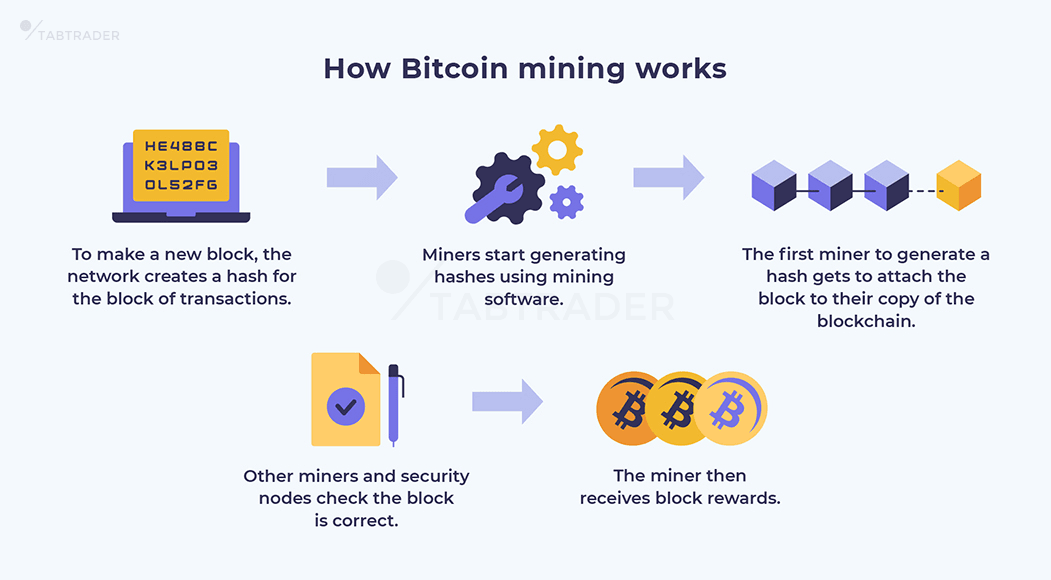
\includegraphics[scale=0.28,clip=false]{pictures/miner.png}
  \end{center}

  \begin{greenbox}{}
    Miners must be powerful computers that remain on almost continously!
  \end{greenbox}

\end{frame}

\begin{frame}\frametitle{Evolution of the miners}

  \begin{center}
    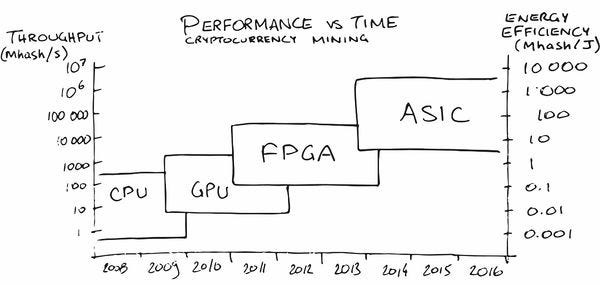
\includegraphics[scale=0.55,clip=false]{pictures/mining-hardware.jpg}
  \end{center}

\end{frame}

\begin{frame}\frametitle{Difficulty over time}

  \begin{center}
    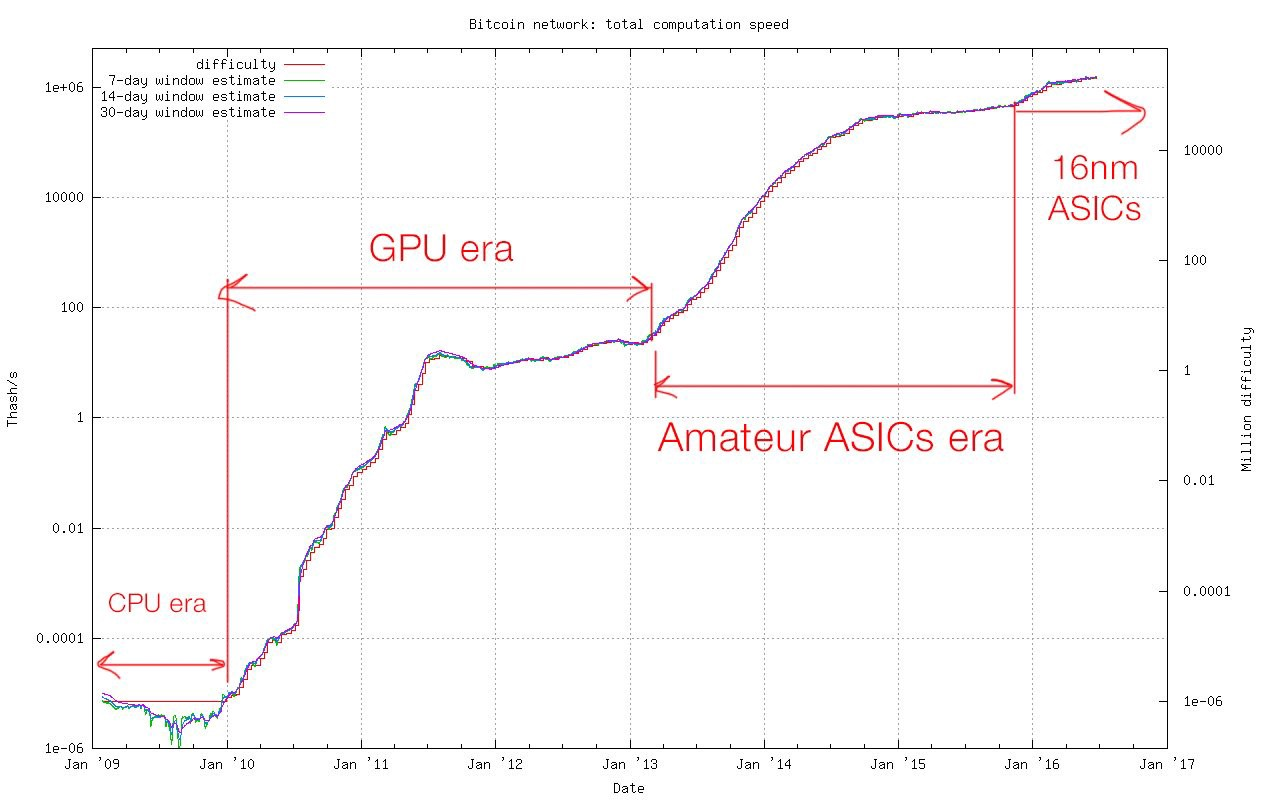
\includegraphics[width=\textwidth,clip=false]{pictures/difficulty.jpg}
  \end{center}

\end{frame}

\begin{frame}\frametitle{PoW costs electricity}

  \begin{greenbox}{2019}
    \begin{center}
      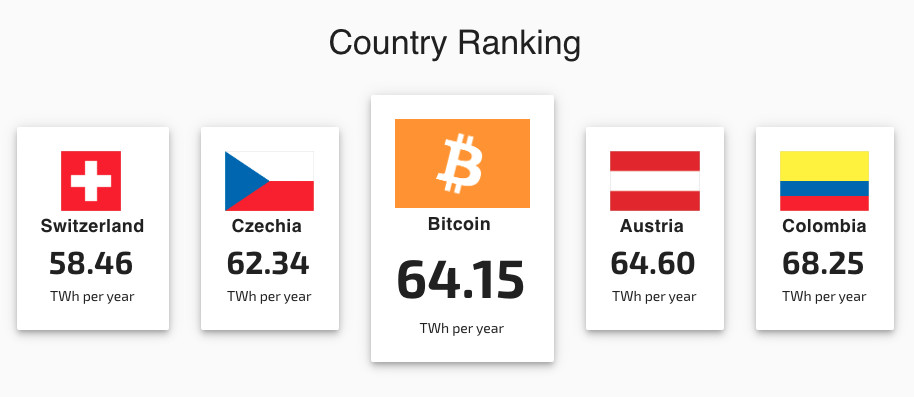
\includegraphics[scale=0.17,clip=false]{pictures/bitcoin-consumption.jpg}
      
\includegraphics[scale=0.14,clip=false]{pictures/greta.jpg}
    \end{center}
  \end{greenbox}
    
\end{frame}

\begin{frame}\frametitle{Blockhains are used for cryptocurrencies}

  \begin{center}
    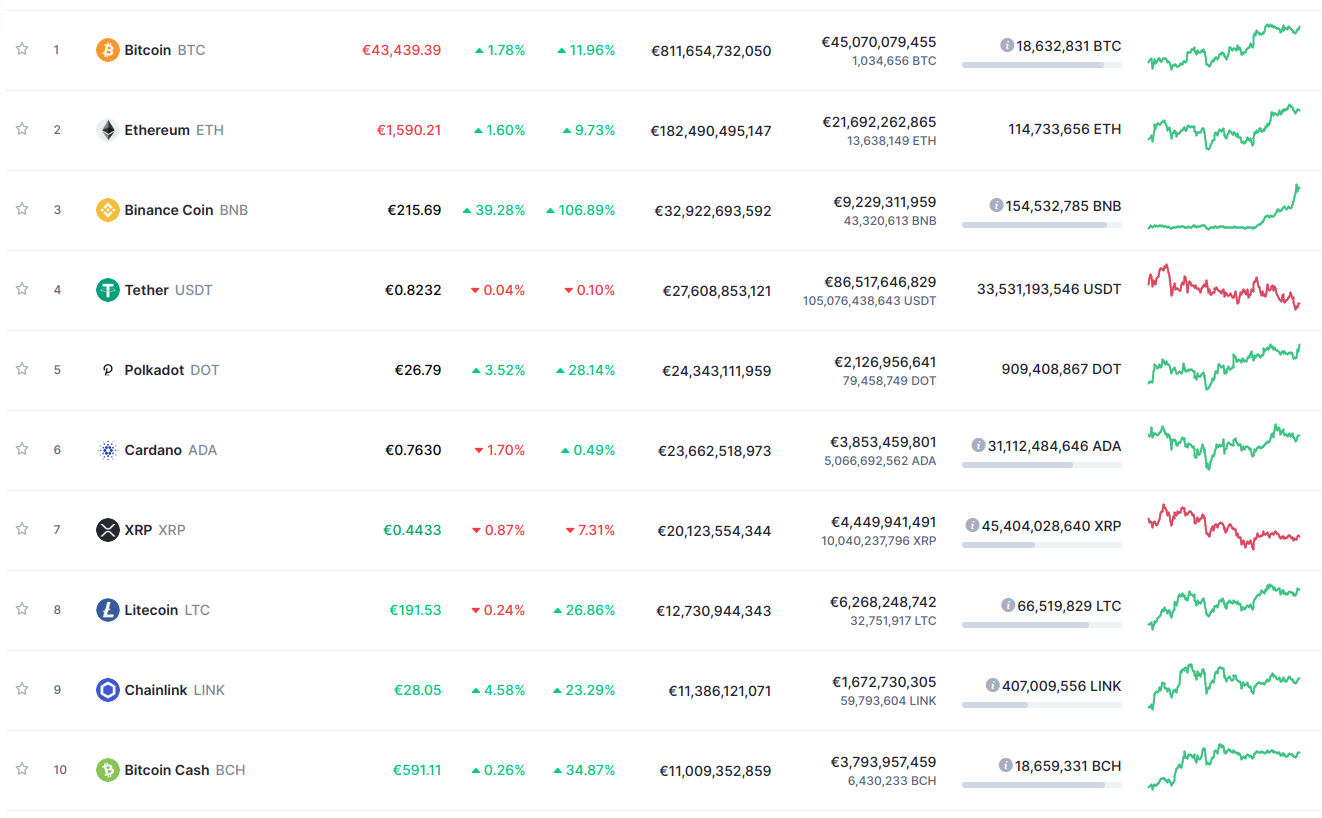
\includegraphics[scale=0.258,clip=false]{pictures/market.png}
  \end{center}

\end{frame}

\begin{frame}\frametitle{Blockhains are used for notarization}

  \begin{center}
    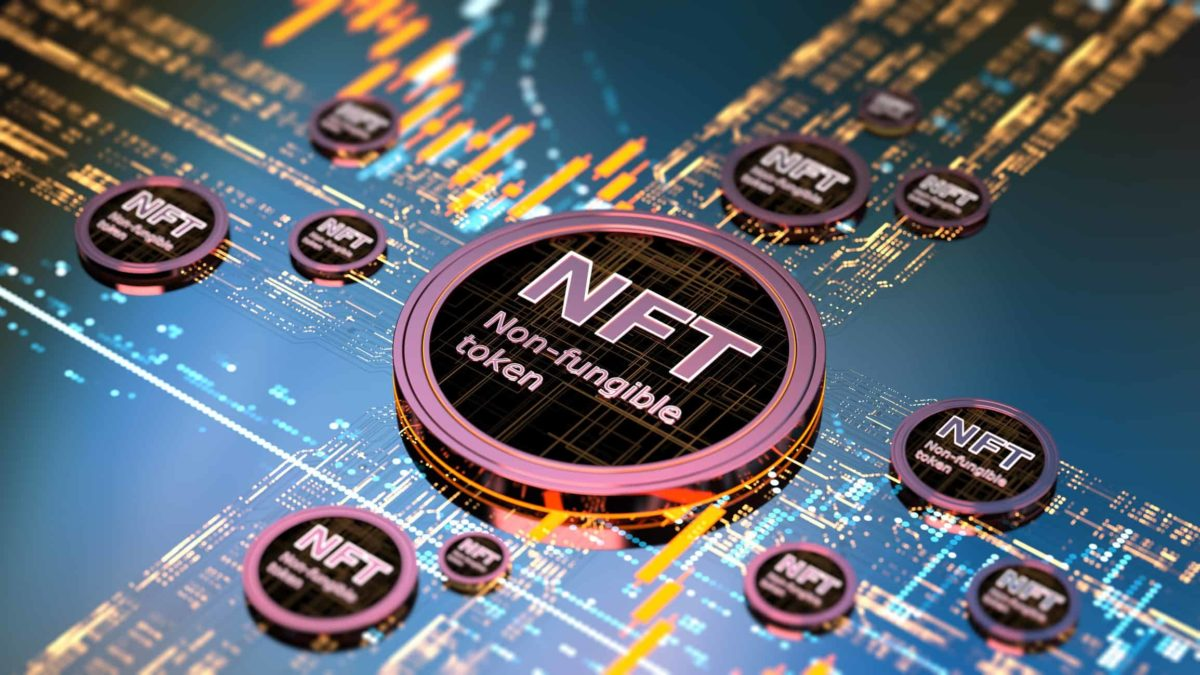
\includegraphics[scale=0.258,clip=false]{pictures/nft.jpg}
  \end{center}

\end{frame}

\begin{frame}\frametitle{Blockhains are used for ransoms}

  \begin{center}
    
\includegraphics[scale=0.7, clip=false]{pictures/ransom.jpg}
  \end{center}

  \begin{redbox}{}
    Send one bitcoin to this account and your data will be decrypted for you
  \end{redbox}

\end{frame}

\begin{frame}\frametitle{Blockhains are used to circumvent international rules or bans}

  \begin{center}
    
\includegraphics[scale=0.5, clip=false]{pictures/send-money.jpg}
  \end{center}

\end{frame}

\begin{frame}\frametitle{Is all this worth its energy consumption and pollution?}

  \begin{center}
    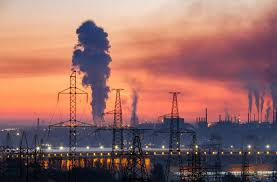
\includegraphics[scale=1, clip=false]{pictures/pollution.jpg}
  \end{center}

\end{frame}

\begin{frame}\frametitle{The best reference}

  \begin{center}
    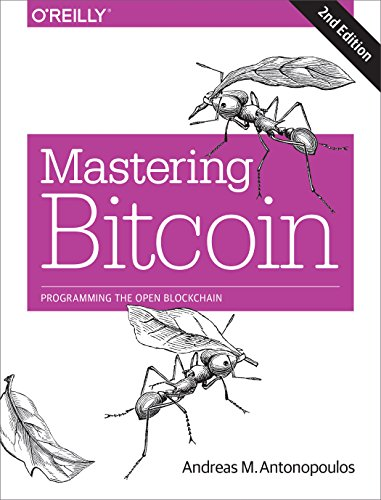
\includegraphics[scale=.35,clip=false]{pictures/mastering-bitcoin.jpg}
  \end{center}

  \begin{center}
    \url{https://github.com/bitcoinbook/bitcoinbook}
  \end{center}

\end{frame}

\begin{frame}
  \frametitle{Can blockchain work without wasting energy?}

  \begin{center}
    Who decides the next block?
  \end{center}

  \bigskip

  \begin{greenbox}{}
    \begin{itemize}
    \item proof of work [PoW] (who works harder and is lucky)
    \item proof of stake [PoS] (who commits more money)
    \item proof of space (who commits more disk space)
    \item proof of authority (who has more authority)
    \item \ldots
    \end{itemize}
  \end{greenbox}

  \bigskip

  \begin{greenbox}{PoS is a variant of Practical Byzantine Fault Tolerance (BFT)}
    Miguel Castro and Barbara Liskov.
    \emph{Practical Byzantine Fault Tolerance and Proactive Recovery}.
    ACM Trans.\ Comput.\ Syst., 20(4):398–461, November 2002
  \end{greenbox}

\end{frame}

\begin{frame}\frametitle{Tendermint (now Ignite): \url{ignite.com}}

  \begin{greenbox}{Jae Kwon. \emph{Tendermint: Consensus without Mining}, 2014.\\
    \url{https://tendermint.com/static/docs/tendermint.pdf}}
    \begin{itemize}
    \item a dynamic set $V$ of validators decides the next block
    \item $V$ might be different for each block
      \begin{itemize}
      \item but deterministically computed from the previous history
      \end{itemize}
    \item at each height $H$, each validator $v\in V$:
      \begin{enumerate}
      \item identifies (deterministically) a validator $p\in V$ that
        is expected to aggregate some transactions and that \alert{proposes} a next block $b$
      \item if $v$ considers $b$ valid, it \alert{pre-votes} $b$
      \item $v$ counts how many validators pre-voted $b$
      \item if $v$ counted at least $\frac{2}{3}$ pre-votes, $v$ \alert{pre-commits} $b$
      \item $v$ counts how many validators pre-committed $b$
      \item if $v$ counted at least $\frac{2}{3}$ pre-commits, $v$ \alert{commits} $b$ and increases $H$
      \item $v$ goes back to step~1
      \end{enumerate}
    \end{itemize}
  \end{greenbox}

  \smallskip

  \begin{center}
    Tendermint is BFT. If step~1 or rewards are based on stakes, then it is PoS
  \end{center}

\end{frame}

\begin{frame}\frametitle{Inside a Tendermint block}

  \begin{center}
    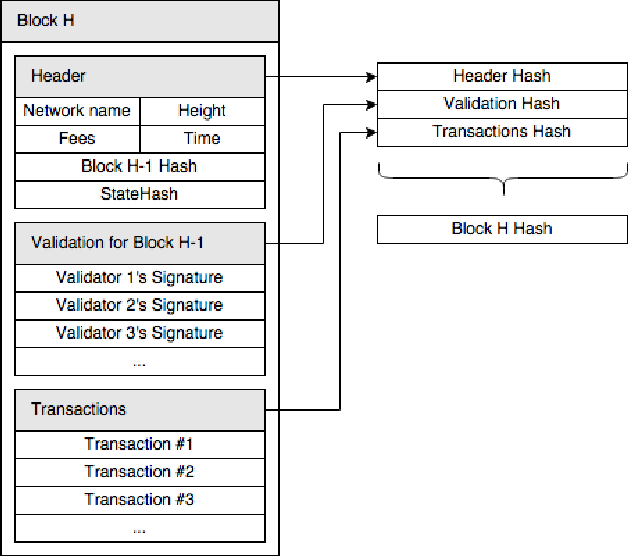
\includegraphics[scale=.38,clip=false]{pictures/tendermint-block.png}
  \end{center}

\end{frame}

\begin{frame}\frametitle{Proof of stake: can we trust it?}

  \begin{greenbox}{Yes we can: Ethereum successfully moved from PoW to PoS}
    \begin{itemize}
    \item it's a special case, whose coin is very valuable: validators are a serious form of investment
    \end{itemize}
  \end{greenbox}

  \bigskip
  
  \begin{redbox}{No we can't: all new blockchain projects use PoS nowadays}
    \begin{itemize}
    \item validators have no interest in being validators (the coin has no value)
    \item validators are afraid of having a machine always connected and open to the internet
    \item validators find it expensive to maintain and update their machine
    \item validators lose cryptocurrency if a blackout or network failure isolate their machine
    \item please ask this question: ``How many validators your blockchain project has, where are they and who maintains such machines'' (spoiler: very few, in the same room, all maintained by a single person)
    \end{itemize}
  \end{redbox}

\end{frame}

\begin{frame}\frametitle{A layered implementation in Golang}

  \begin{center}
    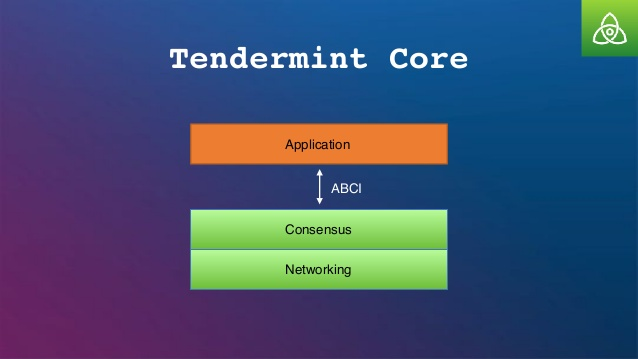
\includegraphics[scale=.45,clip=false]{pictures/tendermint-core.jpg}
  \end{center}

  \begin{center}
    ABCI: Application BlockChain Interface
  \end{center}

\end{frame}

\begin{frame}\frametitle{The ABCI}

  \begin{center}
    \url{https://docs.tendermint.com/master/spec/abci/abci.html}
  \end{center}

  \begin{itemize}
  \item[] \alert{\<checkTx>}: called before entering the mempool and to verify blocks
    \begin{itemize}
    \item[$\Rightarrow$] only transactions that satisfy \<checkTx> are added in blocks
    \item[{
\includegraphics[scale=0.0135]{pictures/uncheck.png}}] must not modify the state of the application
    \end{itemize}
    \hrule
  \item[] \alert{\<beginBlock>}: called at the beginning of a block; receives information
    about the validator set of the previous block and which of them signed the previous block
  \item[] \alert{\<deliverTx>}: called for each transaction added to a block: it executes
    the transaction by modifying the state of the application
  \item[] \alert{\<endBlock>}: called at the end of a block; provides information
    about the validator set for the next block
  \item[] \alert{\<commit>}: called when a block is being committed; provides the hash of
    the state of the application
    \hrule
  \item[] \alert{\<query>}: called when the user wants to read data from the blockchain
  \end{itemize}
\end{frame}

\begin{frame}\frametitle{The database of blocks and the application state}

  \begin{center}
    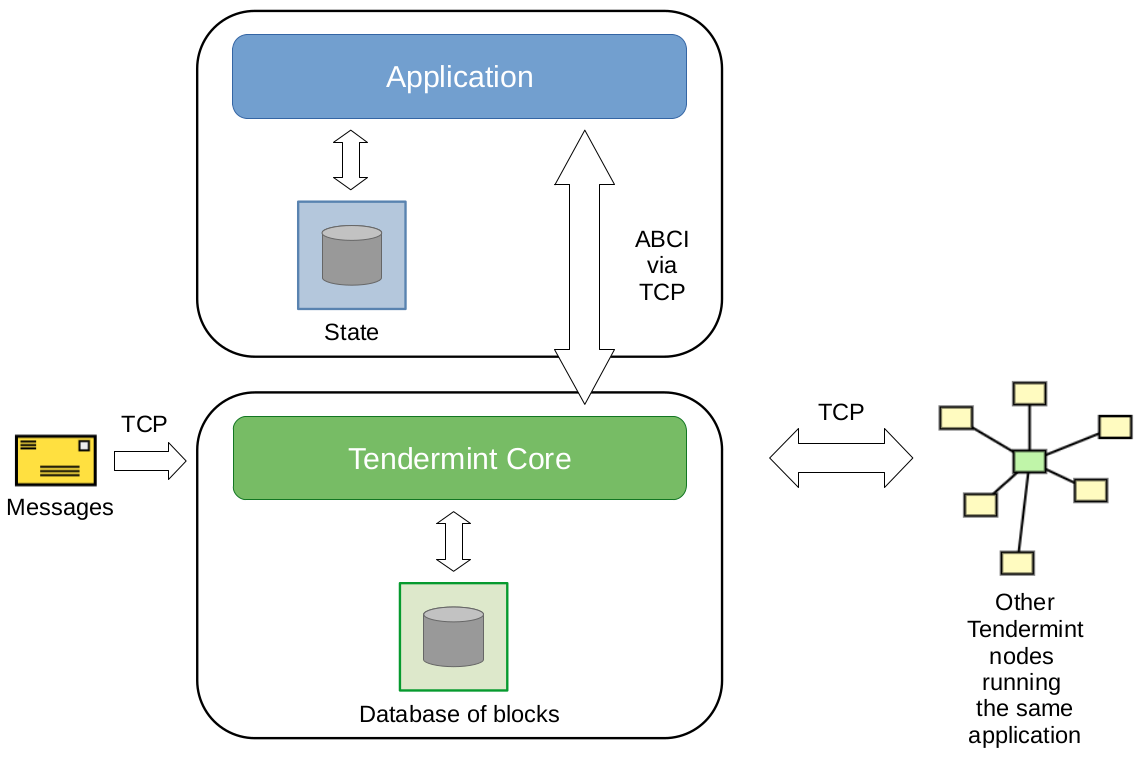
\includegraphics[width=\textwidth,clip=false]{pictures/tendermint-databases.png}
  \end{center}

\end{frame}

\begin{frame}\frametitle{The application state}

  \begin{greenbox}{It must have a function to compute its hash}
    Only that hash is reported in blockchain, for consensus
  \end{greenbox}

  \bigskip

  \begin{greenbox}{It must allow transactional, atomic updates}
    Between \<beginBlock> and \<commit>
  \end{greenbox}

  \bigskip

  \begin{greenbox}{The API of the state}
    Tendermint enjoys finality: there are no forks
    \begin{itemize}
      \item[$\Rightarrow$] one never needs to come
        back in time to the state of a previous block
    \end{itemize}

    \begin{enumerate}
    \item get data
    \item put data
    \item \<h=get\_hash()>
    \item \sout{\<checkout(h)>} $\Rightarrow$ big opportunity for garbage collection!
    \end{enumerate}
  \end{greenbox}

\end{frame}

\begin{frame}\frametitle{Cosmos: a Tendermint application in Golang}

  \begin{center}
    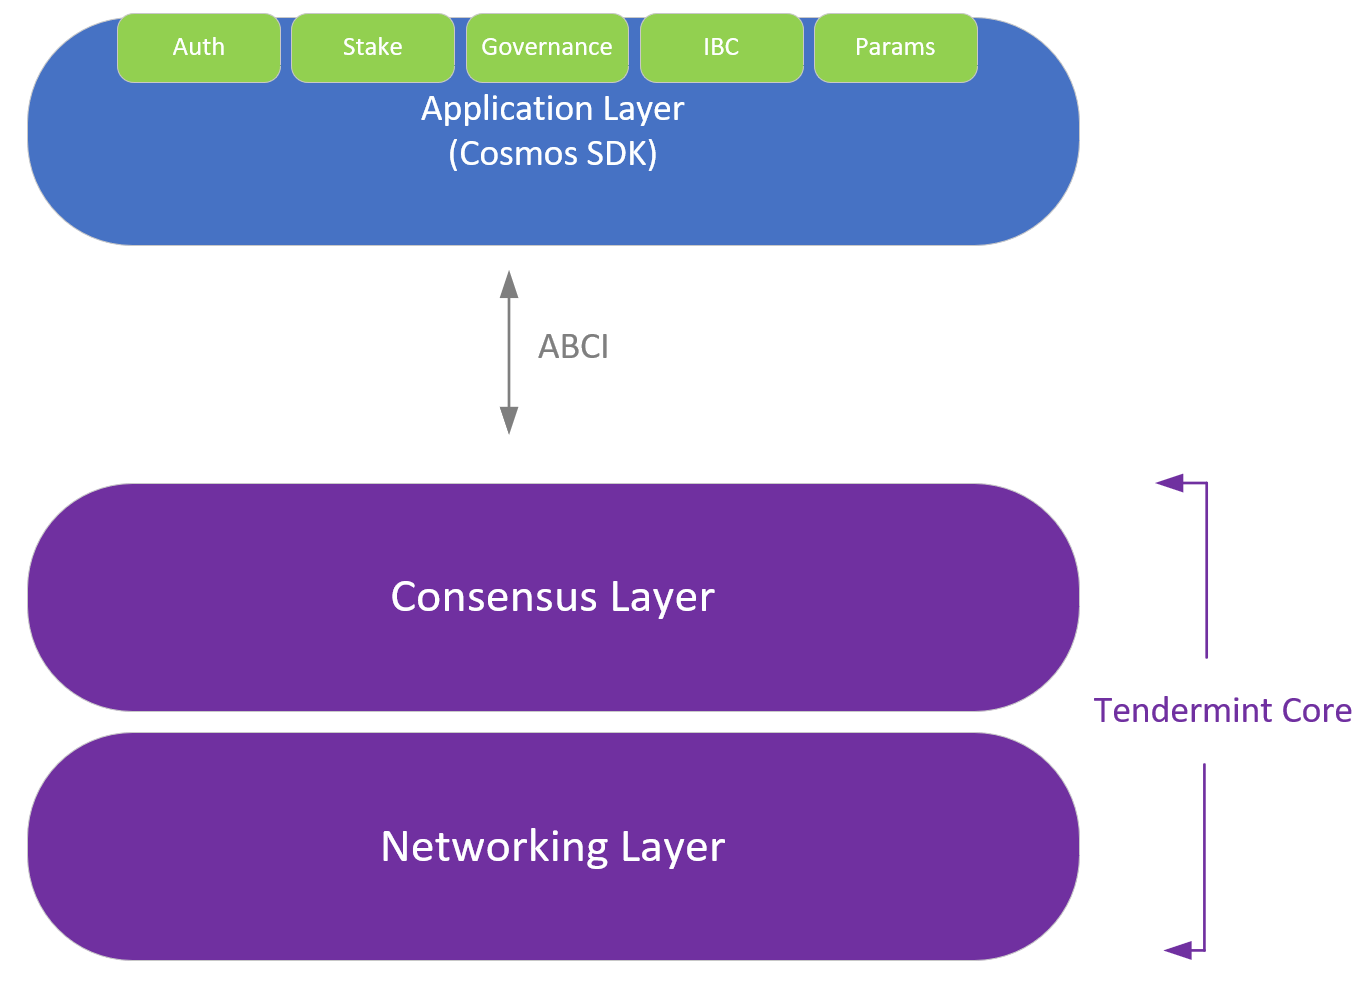
\includegraphics[scale=0.2,clip=false]{pictures/cosmos.png}
  \end{center}

\end{frame}

\section{Hotmoka + Takamaka}

\begin{frame}
  \frametitle{Hotmoka (Fausto Spoto, 2019--2021): \url{www.hotmoka.io}}

  \begin{center}
    
\includegraphics[scale=0.2,clip=false]{pictures/hotmoka_logo.png}
  \end{center}
  
  \begin{greenbox}{}
    An open-source implementation of a network of nodes:
    \begin{itemize}
    \item nodes of a blockchain
    \item IoT devices
    \item computers in the cloud
    \end{itemize}
  \end{greenbox}

  \bigskip

  \begin{greenbox}{Requests are OO-based}
    \begin{itemize}
    \item install code in the node
    \item create an object
    \item call a method of an object
    \item methods are implemented in Takamaka (subset of Java)
    \end{itemize}
  \end{greenbox}

\end{frame}

\begin{frame}\frametitle{Hotmoka nodes \underline{can} be Tendermint applications}

  \begin{center}
    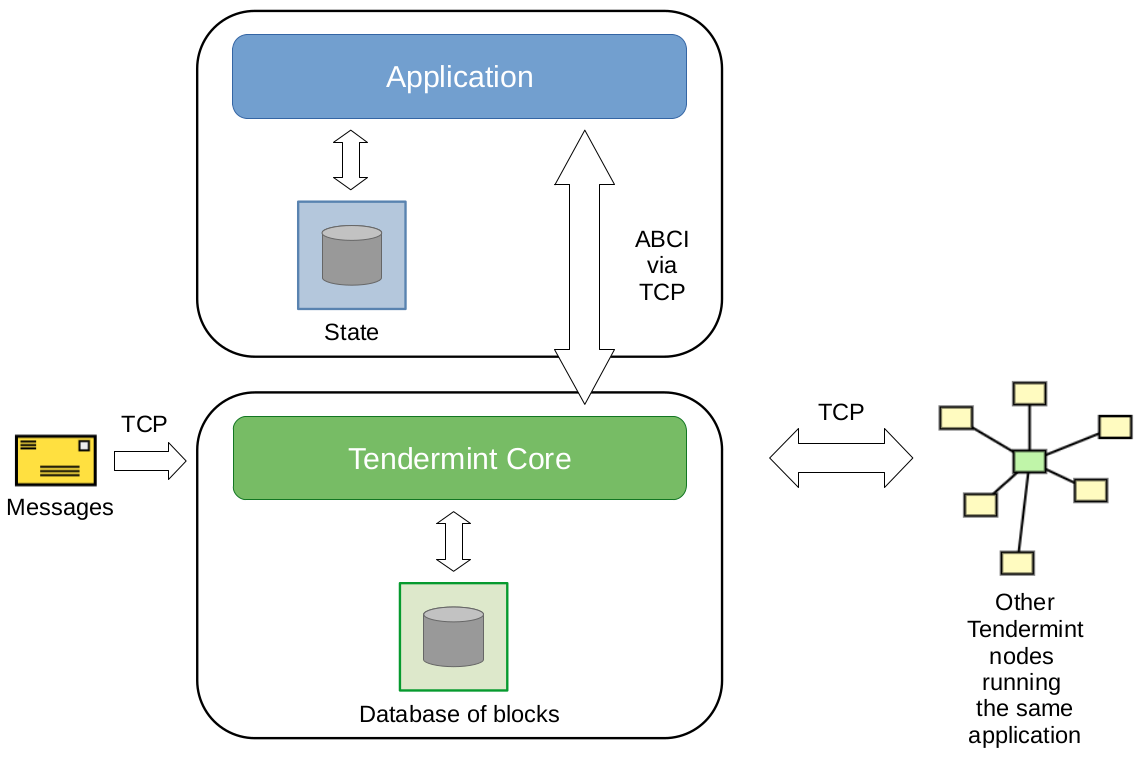
\includegraphics[width=\textwidth,clip=false]{pictures/tendermint-databases.png}
  \end{center}
    
\end{frame}

\begin{frame}\frametitle{An OO state (hash is sha256)}

  \begin{center}
    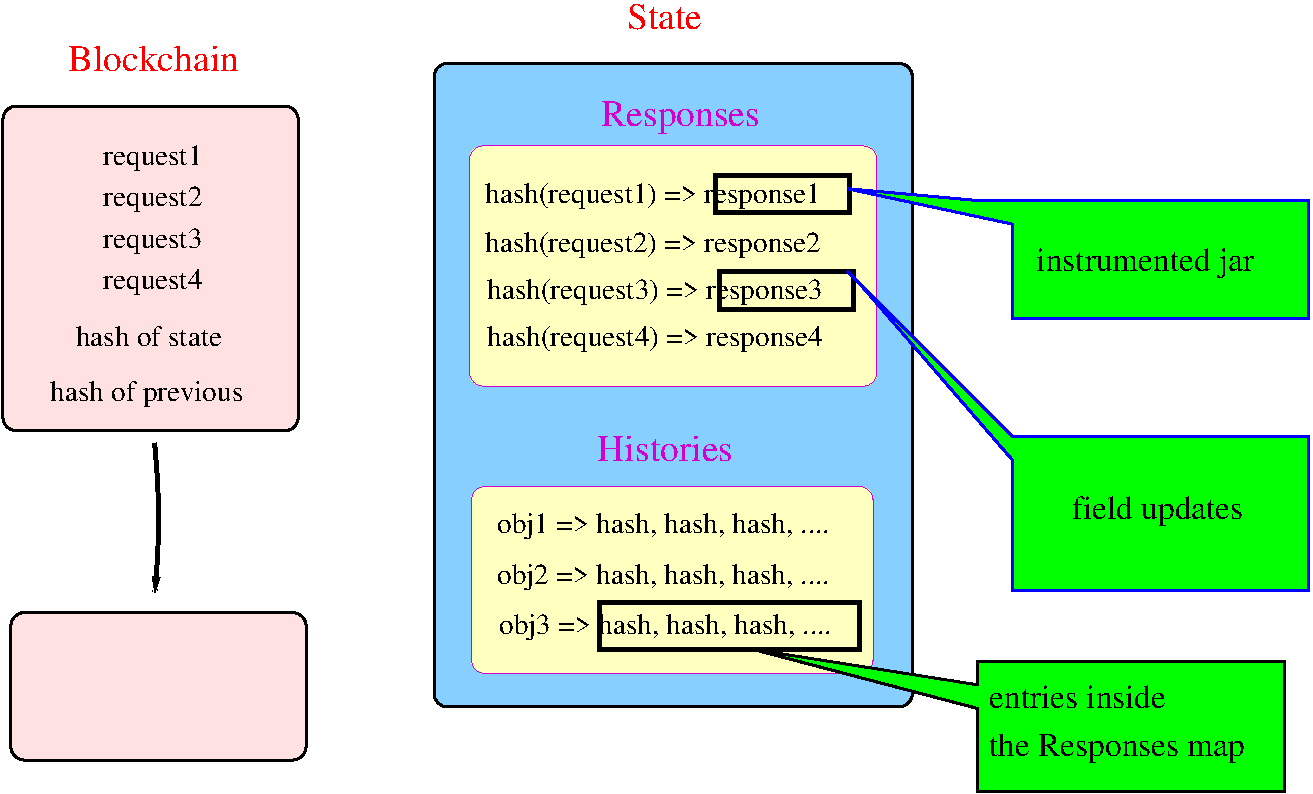
\includegraphics[width=\textwidth,clip=false]{pictures/hotmoka-structure.pdf}
  \end{center}

\end{frame}

\begin{frame}[fragile]\frametitle{The state contains actual Java objects}

  {\scriptsize
    \texttt{manifest:} $\underbrace{{\color{red}\mathtt{42a8a11aee0405aee5775514b3b0456c7740bbb015b4b87df4776e6e4add7668\#0}}}_{\text{machine-independent memory address of an object}}$
  }

  \bigskip

  \begin{greenbox}{{\scriptsize\<moka state 42a8a11aee0405aee5775514b3b0456c7740bbb015b4b87df4776e6e4add7668\#0 --url panarea.hotmoka.io>}}
    {\tiny\begin{semiverbatim}
class {\color{violet}io.takamaka.code.governance.Manifest} (from jar installed at 02dfd29348abaa44f7205251...)
  allowsSelfCharged:boolean = false
  allowsUnsignedFaucet:boolean = true
  chainId:java.lang.String = "chain-ASdWiN"
  gamete:io.takamaka.code.lang.Account = {\color{red}4f7d7ca1fbea152d8f323c21e1abcfa1d979c7c4ea667d8457381a26b08a2d71#0}
  gasStation:io.takamaka.code.governance.GasStation = {\color{red}42a8a11aee0405aee5775514b3b0456c7740bbb015b4b8...}
  maxCumulativeSizeOfDependencies:long = 10000000
  maxDependencies:int = 20
  maxErrorLength:int = 300
  signature:java.lang.String = "ed25519"
  skipsVerification:boolean = false
  validators:io.takamaka.code.governance.Validators = {\color{red}42a8a11aee0405aee5775514b3b0456c7740bbb015b4b8...}
  versions:io.takamaka.code.governance.Versions = {\color{red}42a8a11aee0405aee5775514b3b0456c7740bbb015b4b87df4...}
^ balance:java.math.BigInteger = 0 {\color{violet}(inherited from io.takamaka.code.lang.Contract)}
^ balanceRed:java.math.BigInteger = 0 {\color{violet}(inherited from io.takamaka.code.lang.Contract)}
^ nonce:java.math.BigInteger = 227 {\color{violet}(inherited from io.takamaka.code.lang.ExternallyOwnedAccount)}
^ publicKey:java.lang.String = "" {\color{violet}(inherited from io.takamaka.code.lang.ExternallyOwnedAccount)}
    \end{semiverbatim}}
  \end{greenbox}

\end{frame}

\begin{frame}[fragile]\frametitle{How can Hotmoka identify updates to fields of objects?}

  \begin{greenbox}{The original code}
    \begin{semiverbatim}
      public class C \{
        public {\color{blue}int i;}
        public void foo() \{
          {\color{blue}i} = 42;
        \}
      \}
    \end{semiverbatim}
  \end{greenbox}

  \begin{center}
    No way to know if \<i> changed its value during the execution of \<foo()>
  \end{center}

\end{frame}

\begin{frame}[fragile]\frametitle{How can Hotmoka identify updates to fields of objects?}

  \begin{greenbox}{The instrumented code}
    \begin{semiverbatim}
      public class C {\color{red}extends Storage} \{
        public {\color{blue}int i, old\_i;} // aliased at method start
        public void foo() \{
          {\color{blue}i} = 42;
        \}
      \}
    \end{semiverbatim}
  \end{greenbox}

  \begin{center}
    \<i> changed its value during the execution of \<foo()> iff at the end \<i>$\not=$\<old\_i>
  \end{center}

\end{frame}

\begin{frame}[fragile]\frametitle{How can Hotmoka enforce gas limits?}

  \begin{greenbox}{The original code}
    \begin{semiverbatim}
      public class C \{
        public void foo() \{
          while (...) \{
            ...
          \}
        \}
      \}
    \end{semiverbatim}
  \end{greenbox}

  \begin{center}
    This loop might run for very long or even forever
  \end{center}

\end{frame}

\begin{frame}[fragile]\frametitle{How can Hotmoka enforce gas limits?}

  \begin{greenbox}{The instrumented code}
    \begin{semiverbatim}
      {\color{blue}static long counter;}
      public class C \{
        public void foo() \{
          while (...) \{
            {\color{blue}if (counter++ >= gaslimit)
              throw new OutOfGasError();}
            ...
          \}
        \}
      \}
    \end{semiverbatim}
  \end{greenbox}

  \begin{center}
    Actual gas costs are more fine-grained
  \end{center}

\end{frame}

\begin{frame}\frametitle{Verification and instrumentation of jars in state}

  Each jar that gets installed in a Hotmoka node undergoes two processes:

  \begin{enumerate}
  \item Verification: absence of frequent errors
    \begin{itemize}
    \item objects stored in state extend \<Storage>
    \item non-deterministic or non-terminating library code is not used
    \item no synchronization
    \item no native code
    \item no \emph{dangerous} bytecodes
    \item no finalizers
    \item no static fields (mostly)
    \item code annotations are used correctly
    \item \ldots
    \end{itemize}
  \item Instrumentation
    \begin{itemize}
    \item fields of \<Storage> classes get duplicated
    \item gas metering is weaved into the code
    \item code annotations get implemented \emph{by magic}
    \item \<caller()> is given semantics
    \item \ldots
    \end{itemize}
  \end{enumerate}

\end{frame}

\begin{frame}\frametitle{The Takamaka programming language}

  Takamaka is the subset of Java that passes the verification
  of a Hotmoka node. It uses code annotations to implement contract-based aspects:

  \begin{itemize}
  \item {\color{blue}\<@FromContract>} annotates something that can only be called by a contract,
    not by any other code; hence, it has a {\color{blue}\<caller()>}
  \item {\color{blue}\<@Payable>} annotates something whose execution requires to pay some
    cryptocurrency units
  \item {\color{blue}\<@View>} annotates something whose execution can be run for free,
    without paying for its gas: it must not generate any update at its end
    (\emph{pure} code)
  \end{itemize}

  \bigskip
  Takamaka comes equipped with a {\color{blue}support library}
  (\<io-takamaka-code>) that defines such annotations and
  other typical classes that are useful
  for programming smart contracts (tokens, NFTs, DAOs)

\end{frame}

\begin{frame}[fragile]\frametitle{An example of a Takamaka smart contract}

\vspace*{-1ex}{\tiny\begin{semiverbatim}
{\color{darkblue}{
import static io.takamaka.code.lang.Takamaka.require;
import java.math.BigInteger;
import io.takamaka.code.lang.Contract;
import io.takamaka.code.lang.FromContract;
import io.takamaka.code.lang.Payable;
import io.takamaka.code.lang.PayableContract;
import io.takamaka.code.lang.View;

public class SimplePonzi {\color{red}extends Contract} \{
  private final BigInteger _10 = BigInteger.valueOf(10L), _11 = BigInteger.valueOf(11L);
  private {\color{armygreen}PayableContract} currentInvestor;
  private BigInteger currentInvestment = BigInteger.ZERO;

  public {\color{violet}@Payable} {\color{armygreen}@FromContract(PayableContract.class)} void invest({\color{violet}BigInteger amount}) \{
    BigInteger minimum = currentInvestment.multiply(_11).divide(_10);
    require(amount.compareTo(minimum) >= 0, () -> "you must invest at least " + minimum);

    if (currentInvestor != null)
      currentInvestor.{\color{armygreen}receive(amount)}; {\color{red}// no risk of reentrancy}

    currentInvestor = {\color{armygreen}(PayableContract) caller()};
    currentInvestment = amount;
  \}

  public {\color{red}@View} BigInteger getCurrentInvestment() \{
    return currentInvestment;
  \}
\}
}}\end{semiverbatim}}

\end{frame}

\begin{frame}[fragile]\frametitle{An insurance smart contract in Takamaka}

  \begin{greenbox}{The contract allows one to insure specific days of the year}
    If it rains on those days, one will get an indemnization larger than
    the cost of the insurance
    \begin{itemize}
    \item much larger in summer
    \item just a bit larger in winter
    \end{itemize}
  \end{greenbox}

  \medskip
  The contract provides the following functionalities:

  \begin{itemize}
  \item construction, upon specification of the oracle:
    \[\<{\color{violet}@FromContract} {\color{airforceblue}@Payable} Insurance({\color{airforceblue}BigInteger amount}, Contract oracle)>\]
  \item purchase of an insurance for specific days:
    \[\<{\color{violet}@FromContract(PayableContract.class)} {\color{airforceblue}@Payable} void buy>\]
    \vspace*{-5ex}
    \[\<({\color{airforceblue}long amount}, int day, int month, int year, int duration)>\]
  \item notification of rain and indemnization:
    \[\<{\color{violet}@FromContract} void itRains()>\]
  \end{itemize}
\end{frame}

\begin{frame}[fragile]\frametitle{An insurance contract}

  {\scriptsize\begin{semiverbatim}
public class Insurance extends {\color{blue}Contract} \{
  public final static long MIN = 1_000, MAX = 1_000_000_000;
  private final {\color{blue}Contract} oracle;
  private final {\color{blue}StorageSet}<InsuredDay> insuredDays = new {\color{blue}StorageTreeSet<>()};

  public {\color{violet}@FromContract} {\color{airforceblue}@Payable} Insurance({\color{airforceblue}BigInteger amount}, Contract oracle) \{
    this.oracle = oracle;
  \}

  {\color{red}// inner class}
  private static class InsuredDay extends {\color{blue}Storage} \{ {\color{red}/* not shown */} \}

  public {\color{violet}@FromContract(PayableContract.class)} {\color{airforceblue}@Payable} void buy
    ({\color{airforceblue}long amount}, int day, int month, int year, int duration) \{ {\color{red}/* shown later */} \}

  public {\color{violet}@FromContract} void itRains() \{ {\color{red}/* shown later */} \}
\}
  \end{semiverbatim}}

\end{frame}

\begin{frame}[fragile]\frametitle{Buy an insurance}

{\scriptsize\begin{semiverbatim}
public {\color{violet}@FromContract(PayableContract.class)} {\color{airforceblue}@Payable} void buy
    ({\color{airforceblue}long amount}, int day, int month, int year, int duration) \{

  {\color{armygreen}require(duration >= 1, "you must insure at least one day");
  require(duration <= 7, "you cannot insure more than a week");
  require(amount >= MIN * duration,
    () -> "we insure a single day for at least " + MIN + " units of coin");
  require(amount <= MAX * duration,
    () -> "we insure a single day for up to " + MAX + " units of coin");}

  // if the date is wrong, this generates an exception
  LocalDate start = LocalDate.of(year, month, day);

  PayableContract payer = (PayableContract) {\color{violet}caller()};
  for (int offset = 0; offset < duration; offset++)
    insuredDays.add(new InsuredDay
                    (payer, amount / duration, start.plusDays(offset)));
\}
\end{semiverbatim}}

\end{frame}

\begin{frame}[fragile]\frametitle{Pay the indemnization}

{\scriptsize\begin{semiverbatim}
public {\color{violet}@FromContract} void itRains() \{
  {\color{armygreen}require({\color{violet}caller()} == oracle, "only the oracle can call this method");}

  {\color{red}// pay who insured today}
  insuredDays.stream()
    .filter(InsuredDay::isToday)
    .forEachOrdered(insuredDay ->
          insuredDay.payer.{\color{blue}receive}(insuredDay.indemnization()));

  {\color{red}// clean-up the set of insured days}
  insuredDays.stream()
    .filter(InsuredDay::isTodayOrBefore)
    .forEachOrdered(insuredDays::remove);
\}
\end{semiverbatim}}

\end{frame}

%moka install 251bfca0a37c0cc2611f3a5caee95fedb972e820609c6a0912d2527af53f59bb#0 target/insurance-0.0.1.jar --url panarea.hotmoka.io
\begin{frame}[fragile]\frametitle{On-chain verification: incorrect use of annotations}

  \begin{redbox}{Assume that the programmer forgets the \<FromContract> annotation in \<buy>}
  \<public {\color{green}\sout{@FromContract(PayableContract.class)}} @Payable void buy
  (long amount, int day, int month, int year, int duration)>
  \end{redbox}\pause

  \begin{tt}mvn clean package\end{tt} $\Rightarrow$ regenerates \<target/insurance-0.0.1.jar>\pause

\medskip

\begin{greenbox}{Let's try to install this version of the jar}
{\scriptsize\begin{semiverbatim}
 {\color{red}moka install
 06aa6a1afabc82c7161ffcdc2391a2136101aaeb94f64edd53a1d0d1436d610e\#0
 target/insurance-0.0.1.jar
 --url panarea.hotmoka.io}\pause

Do you really want to spend up to 852500 gas units to install the jar [Y/N] Y
{\color{armygreen}total gas consumed: 852500}
{\color{darkred}  for CPU: 255
  for RAM: 1326
  for storage: 381762
  for penalty: 469157     !!!!!!!}
io.hotmoka.beans.TransactionException:
io.takamaka.code.verification.VerificationException:
{\color{red}it/univr/insurance/Insurance.java method buy:
@Payable can only be applied to a @FromContract method or constructor}
\end{semiverbatim}}
\end{greenbox}

\end{frame}

%moka install 251bfca0a37c0cc2611f3a5caee95fedb972e820609c6a0912d2527af53f59bb#0 target/insurance-0.0.1.jar --url panarea.hotmoka.io
\begin{frame}[fragile]\frametitle{On-chain verification: potential non-determinism}

  \begin{redbox}{Assume to use \<forEach> instead of \<forEachOrdered> in \<itRains>}
\<insuredDays.stream().filter(InsuredDay::isToday).{\color{green}forEach}(...);>
  \end{redbox}\pause

  \begin{tt}mvn clean package\end{tt} $\Rightarrow$ regenerates \<target/insurance-0.0.1.jar>\pause

\medskip

\begin{greenbox}{Let's try to install this version of the jar}
{\scriptsize\begin{semiverbatim}
 {\color{red}moka install
 06aa6a1afabc82c7161ffcdc2391a2136101aaeb94f64edd53a1d0d1436d610e\#0
 target/insurance-0.0.1.jar
 --url panarea.hotmoka.io}\pause

Do you really want to spend up to 852500 gas units to install the jar [Y/N] Y
{\color{armygreen}total gas consumed: 853700}
{\color{darkred}  for CPU: 255
  for RAM: 1326
  for storage: 382362
  for penalty: 469757     !!!!!!!}
io.hotmoka.beans.TransactionException:
io.takamaka.code.verification.VerificationException:
{\color{red}it/univr/insurance/Insurance.java:95:
illegal call to non-white-listed method java.util.stream.Stream.forEach}
\end{semiverbatim}}
\end{greenbox}

\end{frame}

%moka verify target/insurance-0.0.1.jar --libs io-takamaka-code-1.0.0.jar
\begin{frame}[fragile]\frametitle{Off-chain verification}

Using the blockchain as a debugger is very expensive\ldots

\medskip
\begin{tt}
moka verify <jar> --libs dependencies
\end{tt}\pause

\medskip

\begin{greenbox}{We verify the jar off-chain, to find all errors}
{\scriptsize\begin{semiverbatim}
 {\color{red}moka verify
 \only<3>{jar}\only<4->{target/insurance-0.0.1.jar}
 \only<5>{--libs dependencies}\only<6->{--libs io-takamaka-code-1.0.0.jar}}
\onslide<7->{
{\color{red}
it/univr/insurance/Insurance.java method buy:
  @Payable can only be applied to a @FromContract method or constructor
it/univr/insurance/Insurance.java:46:
  caller() can only be used inside a @FromContract method or constructor
it/univr/insurance/Insurance.java:95:
  illegal call to non-white-listed method java.util.stream.Stream.forEach
it/univr/insurance/Insurance.java:99:
  illegal call to non-white-listed method java.util.stream.Stream.forEach
}}
\end{semiverbatim}}
\end{greenbox}

\end{frame}

\begin{frame}\frametitle{ERC20 Tokens}

  \begin{center}
    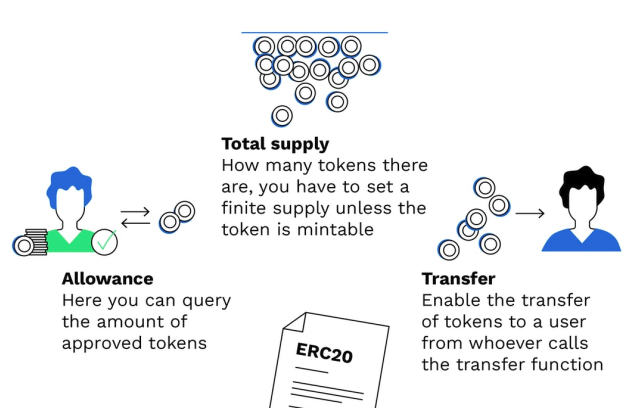
\includegraphics[scale=0.4,clip=false]{pictures/erc20_1.png}
  \end{center}
  
\end{frame}

\begin{frame}\frametitle{ERC20 Tokens}

  \begin{center}
    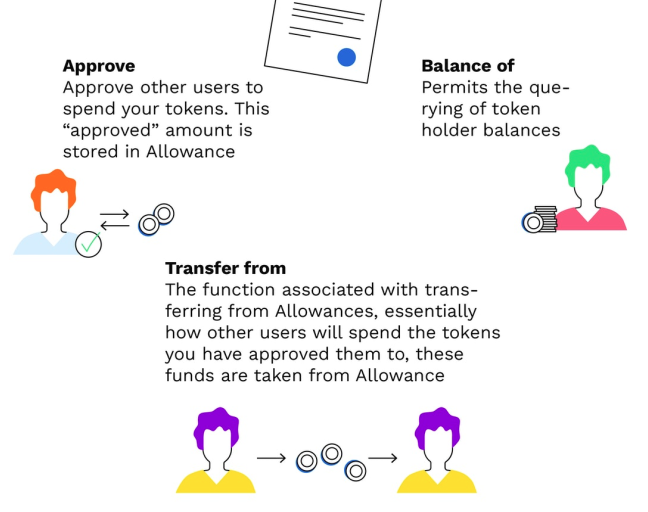
\includegraphics[scale=0.4,clip=false]{pictures/erc20_2.png}
  \end{center}
  
\end{frame}

\begin{frame}\frametitle{The OpenZeppelin reference implementation}

  \begin{greenbox}{We follow (in part) the implementation by OpenZeppelin}
    \begin{center}
      
\includegraphics[scale=0.2,clip=false]{pictures/open-zeppelin.jpg}
    \end{center}
    \begin{center}
      \url{https://docs.openzeppelin.com/contracts/2.x/api/token/erc20}
    \end{center}
  \end{greenbox}
  
\end{frame}

\begin{frame}\frametitle{The hierarchy of the implementation}

  \vspace*{-3ex}
  \begin{center}
    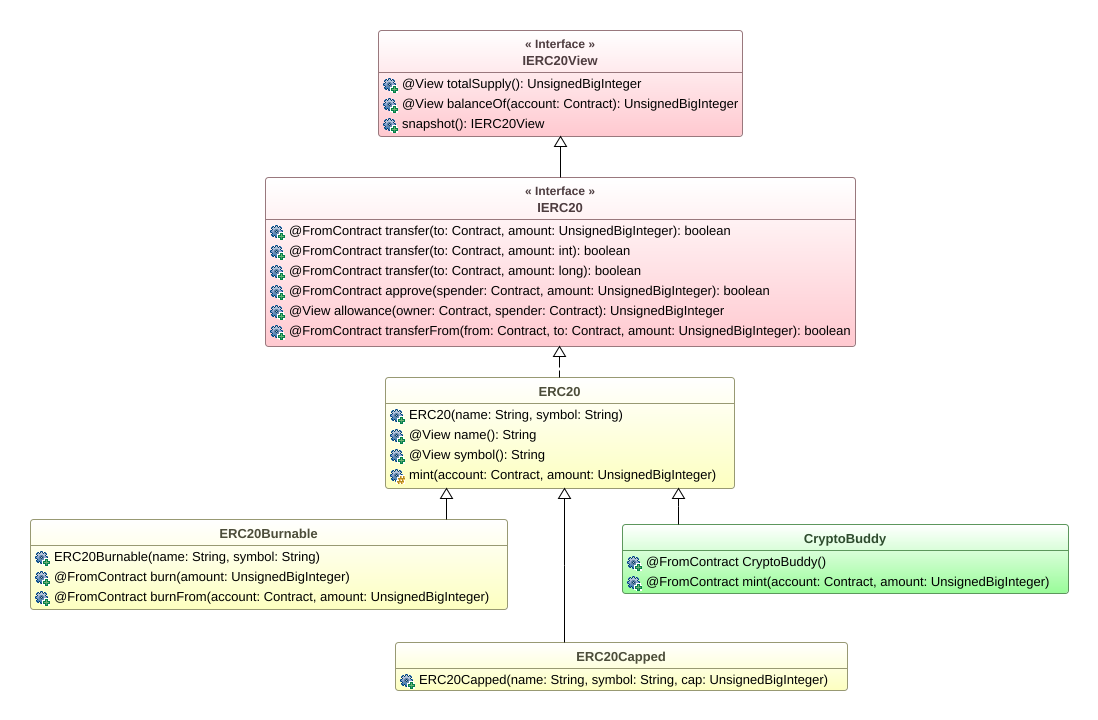
\includegraphics[scale=0.4,clip=false]{pictures/erc20-uml.png}
  \end{center}

\end{frame}

\begin{frame}\frametitle{Inconsistent view}

  \begin{center}
    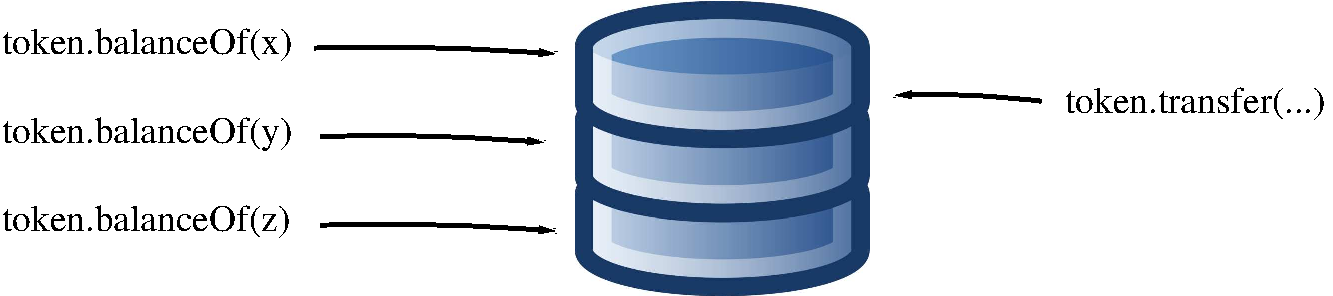
\includegraphics[scale=0.5,clip=false]{pictures/inconsistency.pdf}
  \end{center}

  \bigskip

  Between a call to \<balanceOf> and the next, the state of the token might change in the database
  because other users might call the transfer functions, concurrently

\end{frame}

\begin{frame}\frametitle{Consistent view}

  \begin{center}
    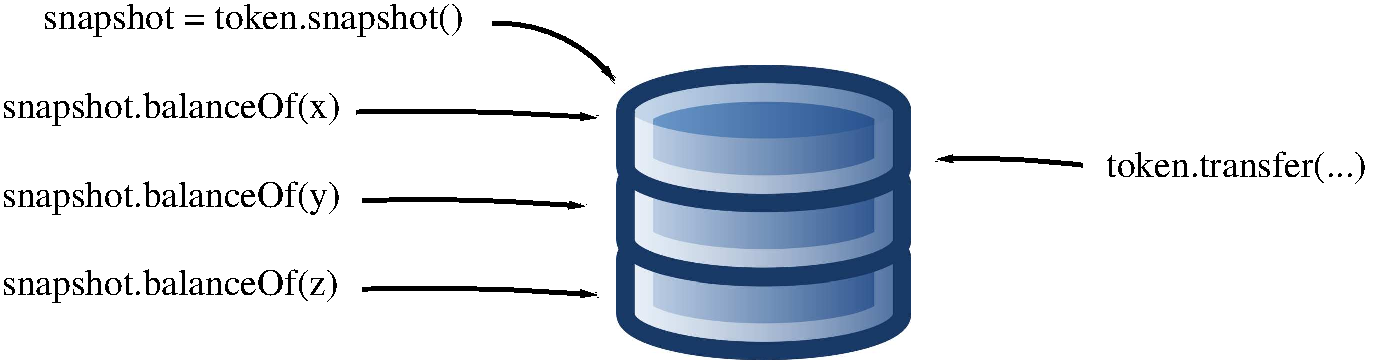
\includegraphics[scale=0.5,clip=false]{pictures/consistency.pdf}
  \end{center}

  \bigskip

  \begin{itemize}
  \item \<snapshot()> works in $O(1)$
  \item all calls to \<balanceOf> refer to the same, consistent state of the token (possibly not the
    latest)
  \item impossible in Solidity, where maps cannot be cloned
  \end{itemize}

\end{frame}

\begin{frame}{References}
  \begin{itemize}
  \item Fausto Spoto:
\emph{A Java Framework for Smart Contracts}. Financial Cryptography Workshops 2019: 122-137
  \item Fausto Spoto:
\emph{Enforcing Determinism of Java Smart Contracts}. Financial Cryptography Workshops 2020: 568-583
  \item Luca Olivieri, Fausto Spoto, Fabio Tagliaferro:
\emph{On-Chain Smart Contract Verification over Tendermint}. Financial Cryptography Workshops 2021: 333-347
  \item Marco Crosara, Luca Olivieri, Fausto Spoto, Fabio Tagliaferro:
\emph{Re-engineering ERC-20 Smart Contracts with Efficient Snapshots for the Java Virtual Machine}. BCCA 2021: 187-194, to appear in Cluster Computing
  \item Andrea Benini, Mauro Gambini, Sara Migliorini, Fausto Spoto:
\emph{Power and Pitfalls of Generic Smart Contracts}. BCCA 2021: 179-186, to appear in Cluster Computing
  \end{itemize}
\end{frame}

\begin{frame}\frametitle{Proof of space}

  \begin{itemize}
  \item proof of work is too expensive and polluting
  \item proof of stake is complex and makes it hard to have many really independent validators
  \end{itemize}

  \medskip

  \begin{greenbox}{Proof of space}
    In 2014, Burstcoin (later Signum) implemented a mining algorithm
    where miners must solve a puzzle to gain the right to mine a new block:
    \begin{itemize}
    \item the puzzle is too hard to be computed for each new block
    \item the puzzle becomes very simple if some information is precomputed and stored on disk
    \item the CPU of the miners remains largely idle: no electricity cost
    \item the more precomputation, the more disk is committed, the higher the probability of solving the puzzle and mining a new block
    \end{itemize}
  \end{greenbox}
  
\end{frame}

\begin{frame}{Mokamint (\url{www.mokamint.io})}

  Signum is monolithic, non-commented, Java 5, undocumented code

  \bigskip
  \bigskip

  \begin{greenbox}{The idea of Mokamint (Fausto Spoto 2023, work in progress)}
    \begin{itemize}
    \item Tendermint: a generic blockchain engine based on proof of stake
    \item Mokamint: a generic blockchain engine based on proof of space
      \begin{center}
        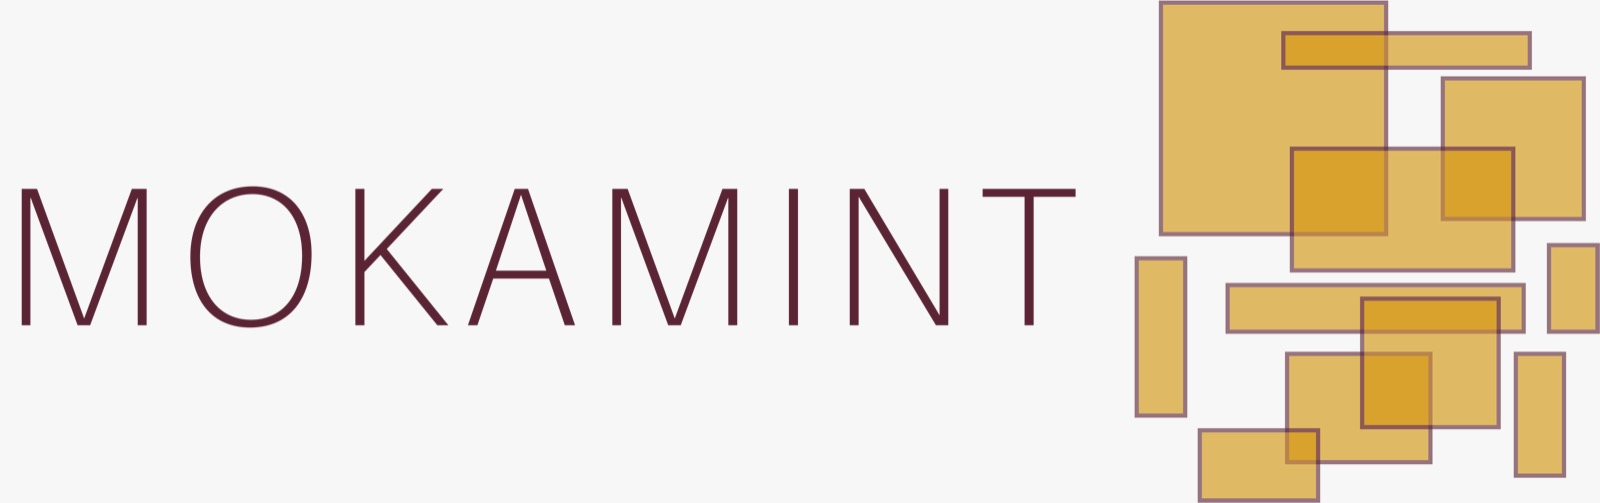
\includegraphics[scale=0.1,clip=false]{pictures/mokamint_colors.jpg}
      \end{center}
    \end{itemize}
  \end{greenbox}

  \bigskip

  Later attach Hotmoka on top of Mokamint, as an application instance

\end{frame}

\end{document}
